\chapter{State of the Art}
\label{cha:state of the art}

\section{Automated and Autonomous Vehicles}

This thesis looks for a way to improve the autonomy of mobile robots. In order to define what qualifies as an improvement in the autonomous behaviour of a mobile robot, one needs to look at the defintion of automated and autonomy. 
The "Expertenkommission Forschung und Innovation" (EFI) defines the term autonomy in the context of robotics as a system which can act without human instructions and still solve complex tasks, make decisions, learn independently aswell as react to unforeseen circumstances \cite{efi2018}. 
The definition specifies the needed requirements to make a robot fully autonomous. 
The automotive industry defines vehicle autonomy in levels based on the human driver's need for supervision and possible intervention during the execution of complex driving tasks \cite{J3016_202104}. Figure \ref{fig:sae_levels} depicts the different levels of autonomy of passenger cars on a scale between no automation to completely autonomous. \\

\begin{figure}[ht]
	\label{fig:sae_levels}
	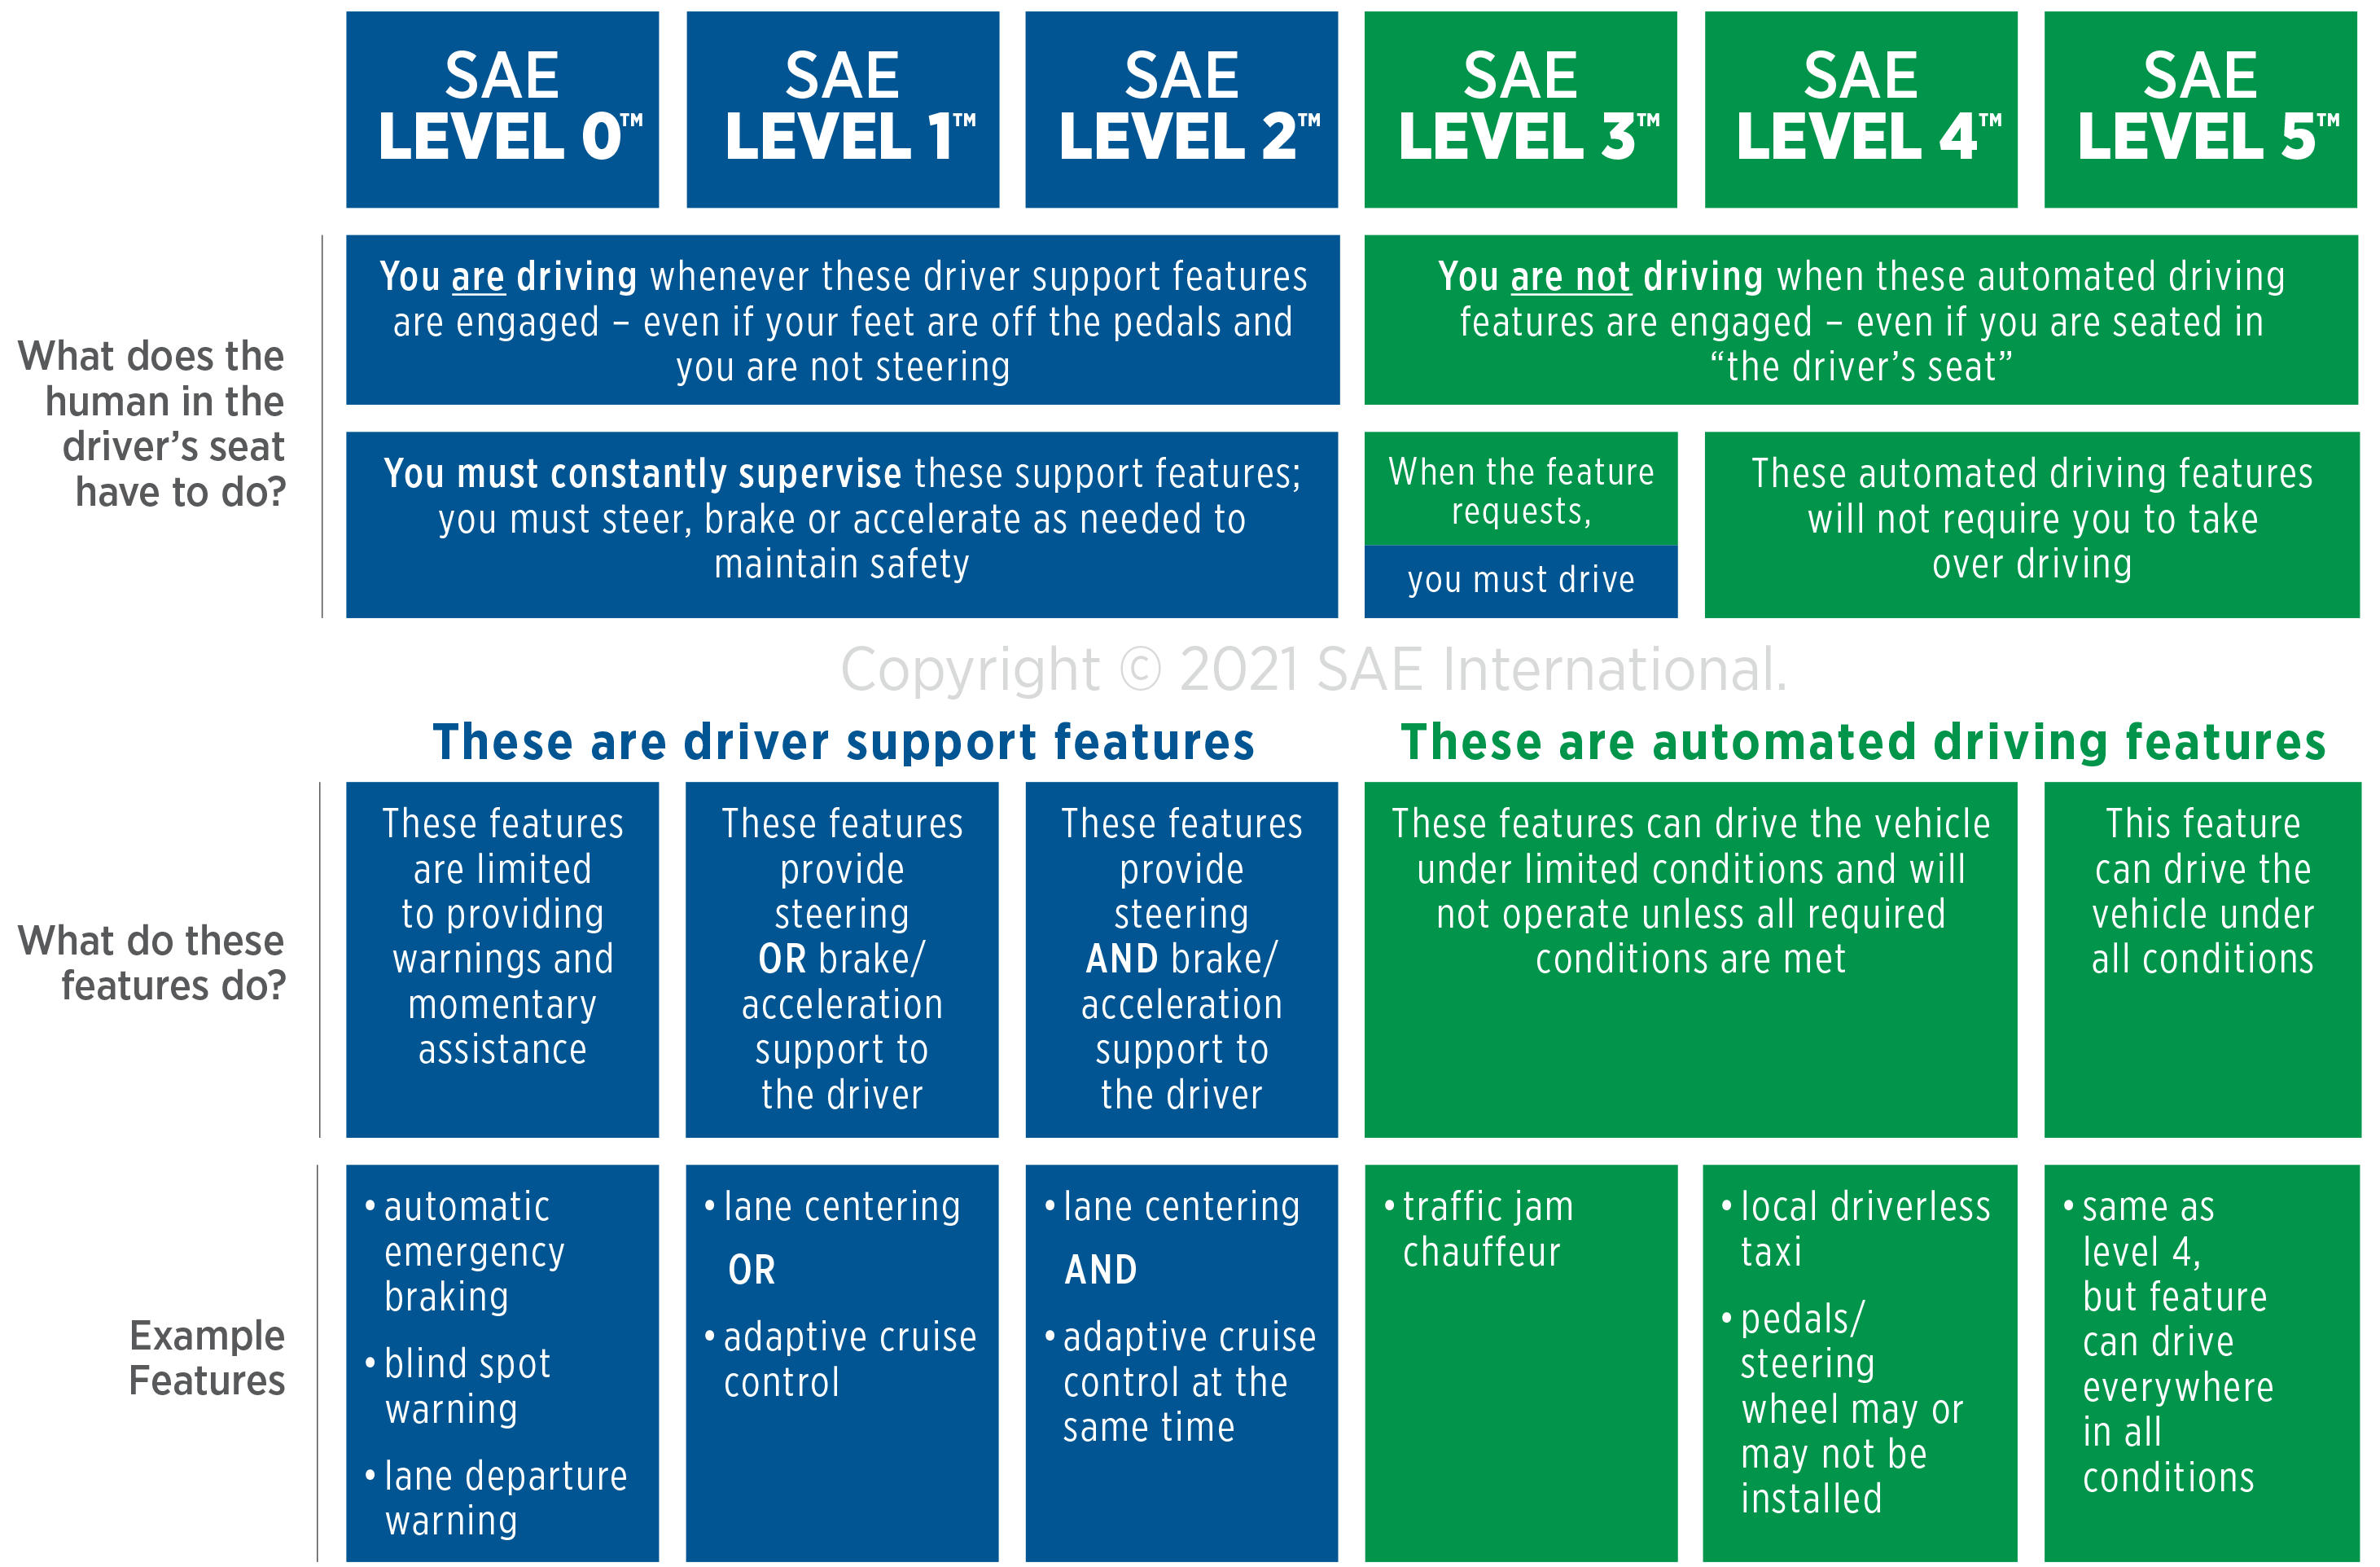
\includegraphics[width=1.0\textwidth]{images/j3016graphic_2021.png}
	\caption{SAE Levels Of Driving Automation \cite{J3016_202104}  }
\end{figure}


Both definitions entail the reliance on human supervision and guidance as the central part of what hinders a system or vehicle to become autonomous. By decreasing the instances a human intervention during the operation of a robot, one can increase the automation level towards full autonomy. But this has to be done by equipping the robot with robust and context-driven decision-making and planning capabilities, otherwise a robot which would never need a human to operate could easily be created. But this robot could not be considered autonomous as it would not able to solve complex tasks and make intelligent decisions.

Different levels of autonomy require different methodologies to achieve them. 



%SAE Levels
%EFI Gutachten
%Fachforum 

\section{Autonomous Driving Navigation Architectures}

To gain a better understanding how behavior planning influences the autonomy of a robot, one can take a look at the latest and most used software architectures for autonomous driving on a functional level. 
Most of the current autonomous driving architectures are implementing a hierarchical structure that follows the "Sense - Think - Act" paradigm \cite{murphy2000}. As shown in figure \ref{fig:autonomous_driving_architecture} the sensory inputs, usually from multiple sensors, get processed to create an environment representation. Then the system calculates how to get from its current position to the destination and creates a path. A second planning calculation is triggered to compute the motion commands with the constraints of the system (e.g. size, turning radius, etc.). These motion commands then get converted to control the motors. 
\begin{figure}[ht]
	\label{fig:autonomous_driving_architecture}
	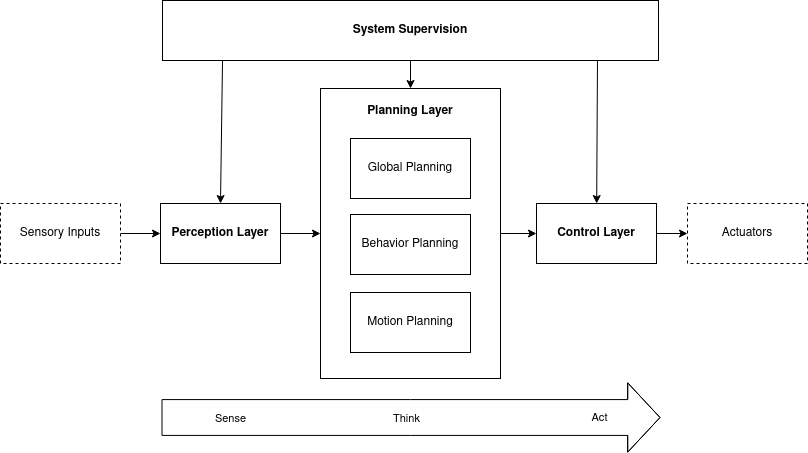
\includegraphics[width=1.0\textwidth]{images/autonomous_driving_architecture.png}
	\caption{Common Autonomous Driving Architecture \cite{brooks1986} \cite{velasco2020}}
\end{figure}
\subparagraph*{}
The planning sequence can be further divided into global planning, behavior planning and local planning. Global planning,also named route planning, is responsible for outputting a path from start to goal. This is comparable to a person using Google Maps to find the shortest or fastest path to a far away city. In this analogy, the behavior planner is responsible to follow the traffic rules on the trip to the destination, e.g. stopping at red lights, giving right of way to other vehicles, following the speed limit. The local planning, also named motion planning, module takes the input from the behavior layer and has the task to let the vehicle drive in accordance to the executed behavior, so that it stays in its lane and comes to a stop at a red light \cite{reke2020}.

\subparagraph*{}
Due to safety considerations, many autonomous driving architectures implement an additional system supervision layer which monitors the execution of the other system components. This supervisor checks the health of all software components. In case one or more components fail to pass the health check the supervisor is responsible for ensuring that the system does not continue the normal driving routine. The supervisor triggers measures to restore the normal functionality or if that is not possible bring the robot into a safe state \cite{zimmermann2020adaptive}. 
Considering that with these architectures, vehicles can achieve an SAE level of autonomy up to level 4 \cite{bacha2008odin},  a good starting point to increase autonomy in a robotic system would be to ensure that all of the functional modules in figure xx are implemented and available. On this basis higher levels of autonomy are achievable through the expansion of the behavior planning module inside of the planning layer. 

%bacha2008
%reke 2020
%wei2014
%brooks1986
%dhillon 2002
%gonzales2016

\section{Behavior Types}

The behavior planning module contains a set of behaviors to operate in a environment. The task of the module is then to choose the best behavior to execute. In this sense a behavior is defined as a mapping of sensory inputs to a pattern of actions that in turn carry out a specific task \cite{murphy2000}. A good behavior planning approach provides the robot with adequate behaviors for every possible scenario the robot is operating in. Different scenarios pose different challenges for the behavior planning module which has to decide on the best behavior option to execute in order to achieve a higher level goal. 

\subsection{Reactive}
During the emergence of behavior based robots, the first type of behavior that was implemented in many robots was a simple reactive behavior. This behavior maps a sensory input directly to motor commands. In human behavior this type of behavior resembles reflexes, like the tapping on the kneecap which unwillingly results in motion in the knee joint. This behavior pattern is not following the typical "Sense, Think, Act" loop, but shortcuts directly from sensing to acting \cite{desilva2008}. Reactive behaviors can be chained together to result in more advanced and goal-driven behaviors. 
\subparagraph*{}
Despite the possibility of more complex robot behaviors, sequential behaviors remain on the level of reactive behaviors due to the lack of a planning and decision-making cycle during their execution. The computational load of reactive behaviours is low and thereby fast as no decision and planning process is taking place, which makes them suited in scenarios where real-time safety is of concern. This property makes these kind of behaviours useful for system supervisor, where sometimes immediate reactions with low latency are required to ensure vehicle safety. But a system with a reactive behavior planning approach will always fail to meet the requirements for higher levels of autonomy due to the fact. This does not mean that reactive behaviors can not be part in highly autonomous systems as their quick response time to sensor inputs makes them valuable in improving vehicle safety and reliability. 


\subsection{Deliberative}
Reactive behaviors suffer the drawback that they are not suitable enable complex behaviors. In addition, the creation of sequences of reactive behaviors that produce the target behavior is a complicated task \cite{murphy2000}. Behaviors that involve a planning and decision making aspect are defined as deliberative. Unlike reactive behaviors, deliberative behaviors are following the Sense, Think, Act paradigm. They are not mapping sensory inputs directly into motor commands. Instead deliberative-type behaviors are deciding the best course of action before acting and only then proceed with the exution. The use of deliberative behaviors in the planning module is what enables a robot to meet the defintion of autonomy, e.g. making decisions and react to unforeseen circumstances. 
\subparagraph*{}
So in order to improve the autonomy of a robot, the focus should be on the creation of deliberative behaviors. A behaviour planner with a deliberative approach makes decision based on current sensor data, as well as previously processed data. By incorporating older sensor information into the decision making process, the deliberative behavior planner can make predictions about the changes that will happen in the environment. This allows the planner to proactively change the motion planning commands to better adapt to the environment. For example, a motion prediction of obstacles in highly dynamic environments would improve the motion planning considerably. This is due to a better understanding of how obstacles are interacting with the planned path of the robot in relation to the time at which the robot and obstacle are predicted to intersect paths. 
\subparagraph*{}
A purely reactive planner could never determine if an obstacle is destined to intersect the robots path in the future and would reroute constantly in order to accomplish the goal. A deliberative planner could determine if the best course of action is to stay on the current path as the dynamic obstacle has already moved away by the time the robot reaches to intersection point. Other actions in scenario are possibly slowing down or speeding up briefly to avoid an obstacle and staying on the current path as this is calculated to be quicker than rerouting and taking a longer path. 
Generally, these cognitively more complex behaviours mimic human skills and thus make a system more autonomous. 

%\textit{Talk about machine learning as deliberative behavior -> true autonomy bc learning and unknown scenarios, programmers can not cover every scenario, so a well designed/trained ai is needed to make a system really autonomous, but -> missing determinism and unaccountability of machines, hence we need behaviors that are still hard coded and deterministic, these can be highly automated. traditional behaviour  and ai generated behaviours can and must coexist in the system (adler2019)}
%
%silva2008
%ingrand 2014
%vasiolopolous 2022

\subsection{Hybrid}
To create reliable aswell as intelligent systems one can combine reactive and deliberative behaviours in a hybrid model. This behavior planning module is then able to quickly react to incoming sensor data and still exhibit high levels of automation. 

\begin{figure}[ht]
	\label{fig:hybrid_planning}
	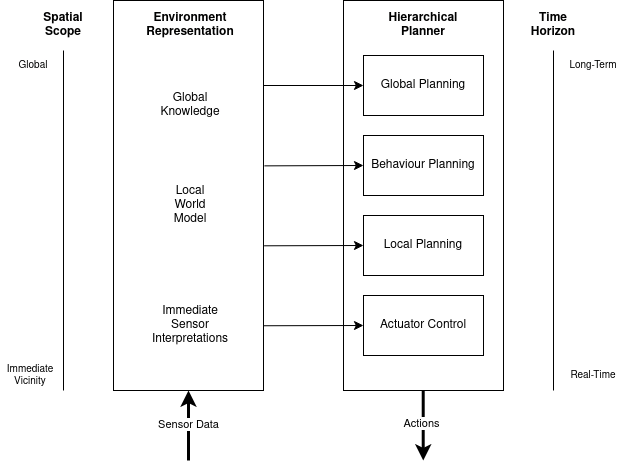
\includegraphics[width=1.0\textwidth]{images/Deliberative_hierarchical_planning.png} 
	\caption{Hybrid Planning Architecture \cite{arkin1998}  }
\end{figure}

Figure \ref{fig:hybrid_planning} shows the areas where reactive and deliberative behaviours have their advantages and limitations. Deliberative planning does possess limitations during the execution of generated plans as the time horizon is long-term and not able to react to fast changes in the environment . When the system is not adressing these points, deliberative robots are very focussed on a small problem domain and are not robust \cite{arkin1998}.
The incorporation of reactive behaviors into the behavior planning combats this problem. In this multi-layer approach the higher level, more deliberative planners are able to override the reactive planners in order to allow the system to be more flexible and adaptible but still maintain fast reaction times. 
This architecture leads to more robust robots that are able to be deployed in a wider variety of environments, thus leading to higher levels of autonomy.


\section{Behavior Planning Approaches}

Robots that use a hybrid, hierarchical behavior planning approach need a system which decides on a high level which behaviors are to be executed. This allows overriding simple reactive behaviors with more complex, deliberative behaviors when the system benefits from it. 

The different solution for such behavior execution system all share the fact that they make use of states a robot can be in. Based upon a robots state and additional information about the environment, different strategies and behaviors are executed during the runtime of the system. 
 

\subsection{Finite State Machines}

Finite State Machines (FSM) are commonly used in the environment of autonomous driving. They are used to describe behavior in a form of states, which in turn execute action. A finite state machine is defined by a list of possible states S, a starting state s0, a set of state transitions delta, a set of final states F and the input alphabet sigma. At any given time only a single state is selected and its containing actions are executed. 

\begin{figure}[ht]
	\label{fig:fsm}
	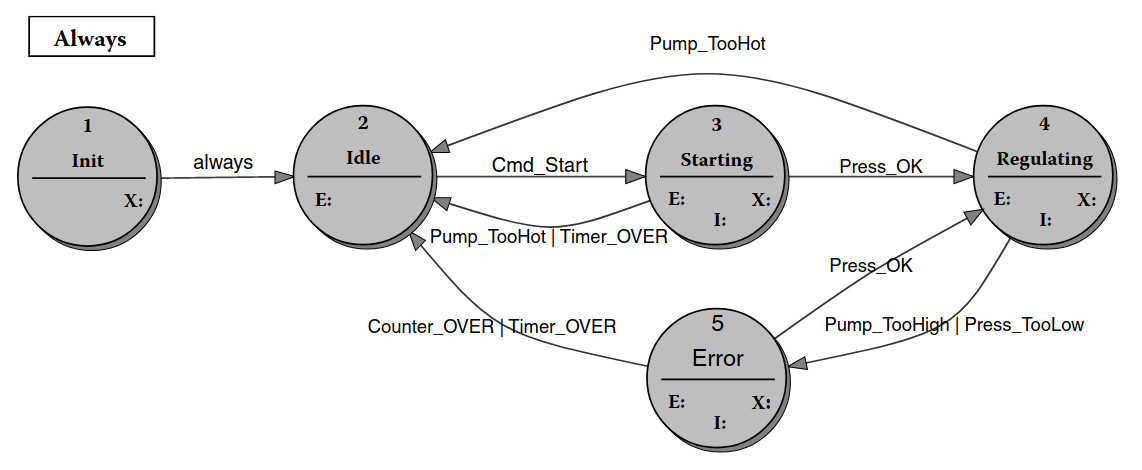
\includegraphics[width=1.0\textwidth]{images/fsm.png} 
	\caption{Example of a finite state machine transition diagram \cite{wagner2006} }
\end{figure}

\subparagraph*{}
Figure \ref{fig:fsm} depicts an example state machine with different states and examplatory transitions between them. Inside of the states the letters indicate the existence of actions.  E stands for entry, I for Input and X for Exit. The arrows between the states illustrate the possible transition and transition conditions for every state. A state transition diagram is a good way to understand the system behavior but can not show the details of the modedeled behavior, like the actions \cite{wagner2006}. 
\subparagraph*{}
Creating small state machines can easily and quickly be accomplished through the use of various feature-rich and performant libraries \cite{fourakis2014}. 
Finite state machines are often being used for comprehensive modeling of reactive behavior and sequential behaviors in autonomous driving functions \cite{ziegler2014}. These finite state machines make use of nested state machines inside of another state machine. This reduces the complexity of the state machine as the transition do not need to be modeled, because the start and final state of a nested state machine is treated as just one state inside of the larger state machine. Despite this possibility to simplify state machines, as a modeled behavior system grows larger to accomodate more complex behaviors into the state machine the effort to expand and maintain the state machine grows rapidly. This is due to the modeling effort of the transitions, transition conditions and transition events growing with each new state that gets introduced into the state machine as existing states need to be checked and updated accordingly \cite{conner2017}. 
\subparagraph*{}
The execution time of finite state machines can be fast enough that they are used to control the motors of a bipedal robot to enable the robot to balance and walk despite unexpected height variations between steps \cite{park2013}. This property makes state machines suited very well suited for fast, reactive type behaviors and still allows a hierarchical approach to behavior planning.


%
%allgeuer 2013
%connor 2017
%ziegler 2014

\subsection{Behavior Trees}
Behavior Trees (BT) are another way to model and control the behavior of autonomous systems. Behavior Trees first found big acceptance in the computer game industry where they are mainly used to model artificial intelligence for non-player characters \cite{florez2009}. Every tree consists of one root and many child, parent and leaf nodes. Leaf nodes are also called execution nodes, while non-leaf nodes are called control or control flow nodes. 
\subparagraph*{}
The execution of a behavior tree is done by ticking the root node of tree. This signal then travels down to the child node of the root node, where either control nodes are being ticked or action nodes are executed. Nodes return either "Success", "Running" or "Failure" which influences how the tick signal gets processed by the rest of the behavior tree. Control nodes can be of the type "Sequence", "Fallback" or "Condition". The condition node can not have child nodes and can only return success or failure. A sequence node can be compared to a logical "and" condition. This means that once a sequence gets ticked from the parent node, it will send the tick signal to every child node as long as they return "success" of "running", and only return "success" itself when every child node was successfully ticked. If any of the child nodes return "failure", the sequence node will stop ticking the remaining children and return "failure". On the other hand the fallback node is an equivalent of a logical "or" condition. The fallback node will tick its child nodes as long as they return "failure" or "running" and will return "success" if one of the ticked node returned "success". It will only return "failure" if all of the child nodes "returned success". All of the basic node types and their control flow modification are listed in table \ref{tab:node_types}.

\begin{table}[ht]
	\label{tab:node_types}
	\caption{The five types of nodes \cite{iovino2022}}
	\begin{tabular}{ | m{0.13\textwidth} | m{0.13\textwidth}| m{0.2\textwidth} | m{0.2\textwidth} | m{0.2\textwidth} |} 
  	\hline
  	Node type & Symbol & Succeeds & Fails & Running \\ 
  	\hline
  	Sequence & -$>$ & If all children succeed &  If one child fails & If one child returns running \\ 
  	\hline
  	Fallback & ? & If one child succeeds & If all children fail & If one child returns running \\ 
  	\hline
  	Parallel & -$>$ -$>$ & If $>$= M children succeed & If $>$ N-M children fail & else \\
  	\hline
  	Action & shaded box & Upon completion & When impossible to complete & During completion \\
  	\hline
  	Condition & white oval & If true & If false & Never \\
  	\hline
	\end{tabular}
\end{table}


Figure \ref{fig:bt_example} depicts an example of a BT with multiple levels and action nodes. The nodes with the arrow (-$>$) symbol are sequence nodes, the question mark (?) symbol denotes fallback nodes. The condition node are depicted as white ovals. The action nodes are represented as gray rectangles in the BT example.

\begin{figure}[h!]
	\label{fig:bt_example}
	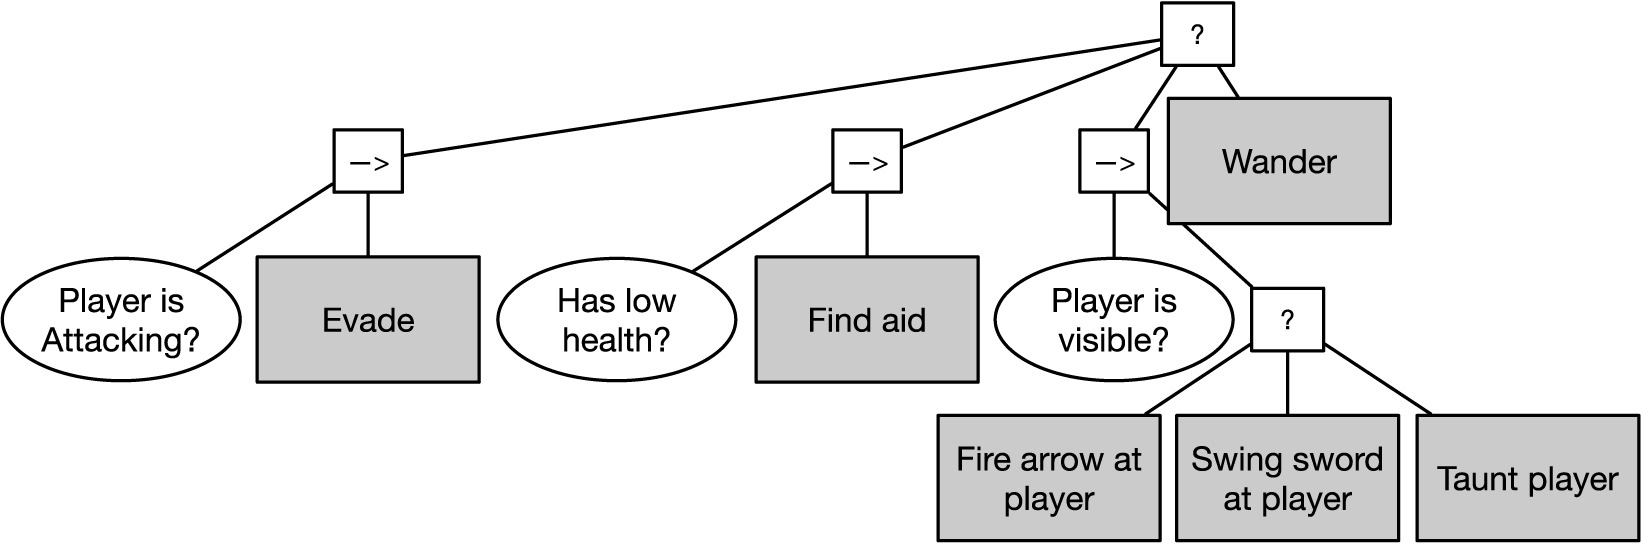
\includegraphics[width=1.0\textwidth]{images/bt_example.jpg} 
	\caption{Example of a behavior tree \cite{iovino2022} }
\end{figure}

One of the core differences to Finite State Machine is that transitions between states are not distributed across all the states but they are organized in a hierarchical tree, where the leaves are representing the states \cite{iovino2022}. While both FSM and BT are capable of producing the same behavior in robots, the fundamental shift in how the two system are created lead to significant advantages in the modularity, synthesis and analysis of the systems at hand. These effects are more significant with an increase in size of the system. BT offer a lot more flexibility when creating an advanced behavior layer for an autonomous system. 


%iovino2022
%marzinotto 2014
%colledanchise 2018

%\subsection{POMPDs}

% \section{Deterministic Behavior}


